\section{Конструкторская часть}

В данном разделе будут рассмотрены схемы алгоритмов обновления гипертекстового документа с использованием DOM, VDOM и алгоритма согласования, а также алгоритма Fiber.
Также будут найдены их трудоёмкости и произведено их сравнение на основе полученных результатов.

\subsection{Разработка алгоритмов}

На рисунках \ref{fig:dom-algorithm}--\ref{fig:child-reconciliation-algorithm}, представлены схемы алгоритмов обновления документа с использованием DOM, VDOM, а также алгоритма согласования соответственно, разработанных на основании приведённых в части \ref{analysis} описаниях.

\begin{figure}[h]
	\centering
	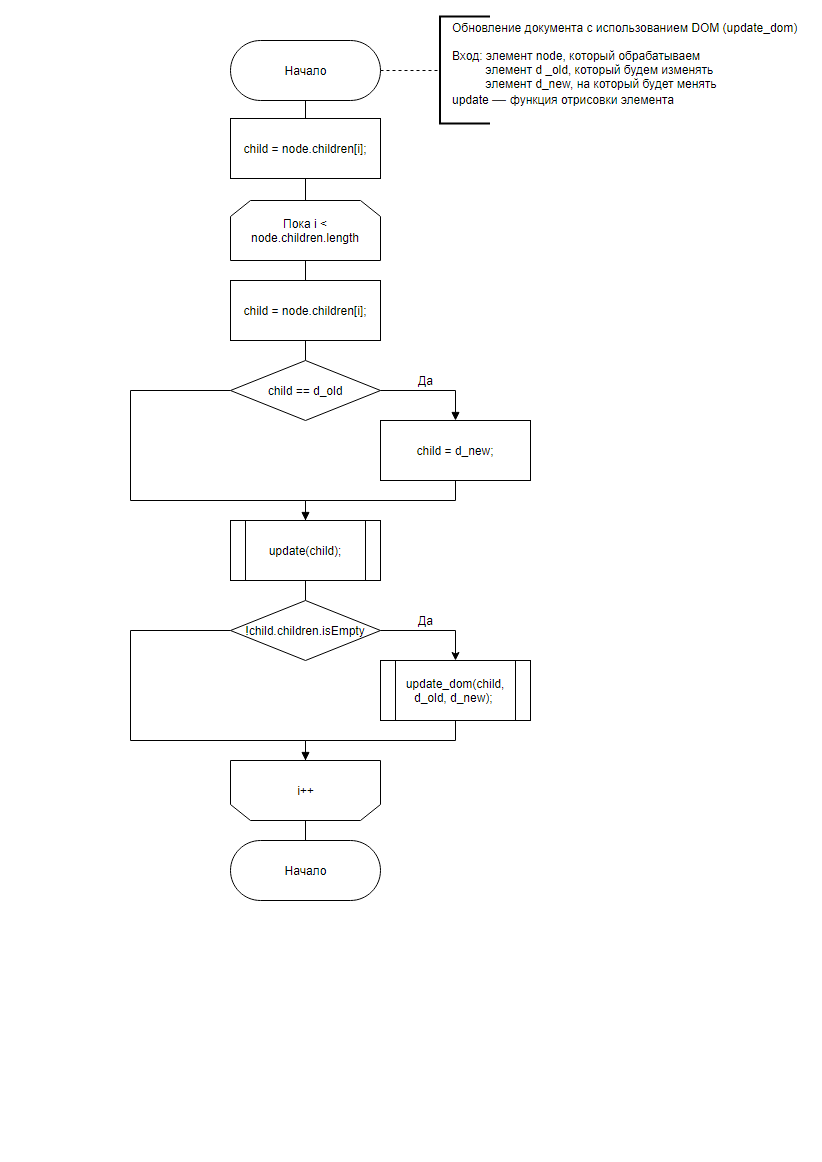
\includegraphics[width=170mm]{img/dom-algorithm.png}
	\caption{Схема алгоритма обновления документа с использованием DOM}
	\label{fig:dom-algorithm}
\end{figure}

\begin{figure}[h]
	\centering
	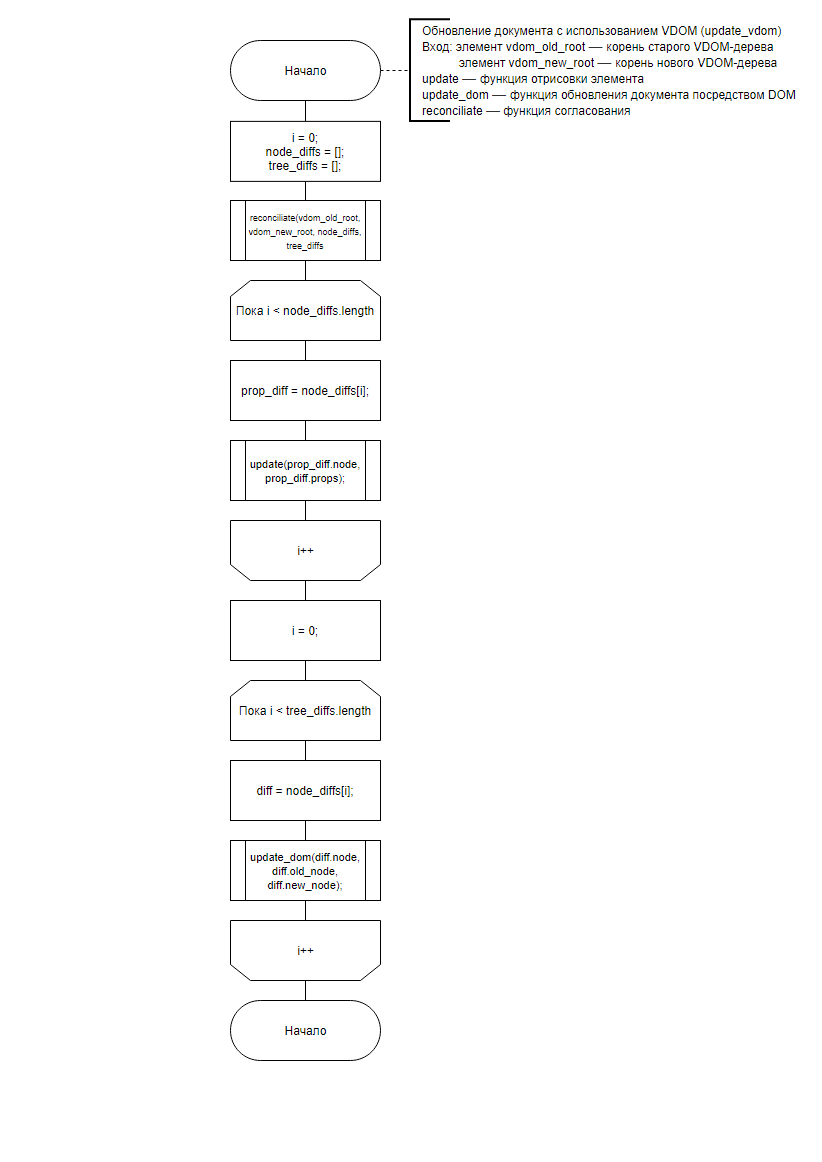
\includegraphics[width=170mm]{img/vdom-algorithm.png}
	\caption{Схема алгоритма обновления документа с использованием VDOM}
	\label{fig:vdom-algorithm}
\end{figure}

\begin{figure}[h]
	\centering
	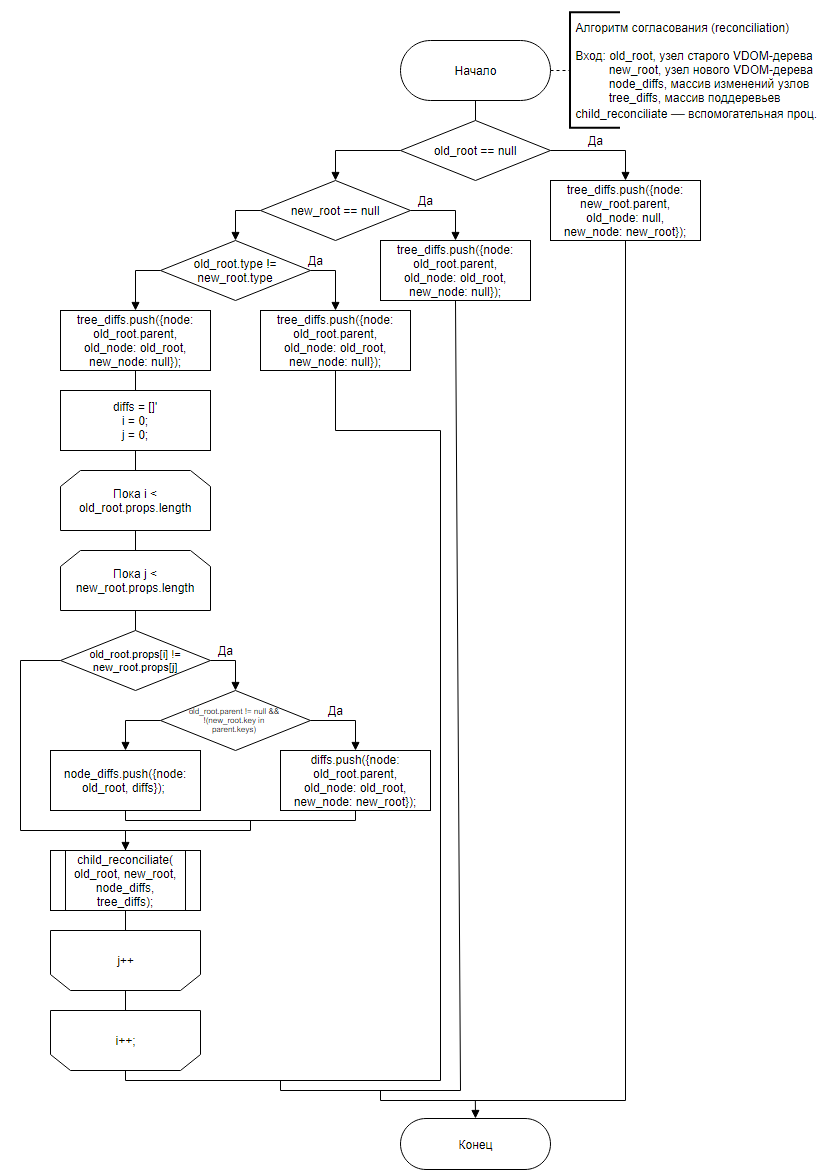
\includegraphics[width=170mm]{img/reconciliation-algorithm.png}
	\caption{Схема алгоритма согласования, часть 1}
	\label{fig:reconciliation-algorithm}
\end{figure}

\begin{figure}[h]
	\centering
	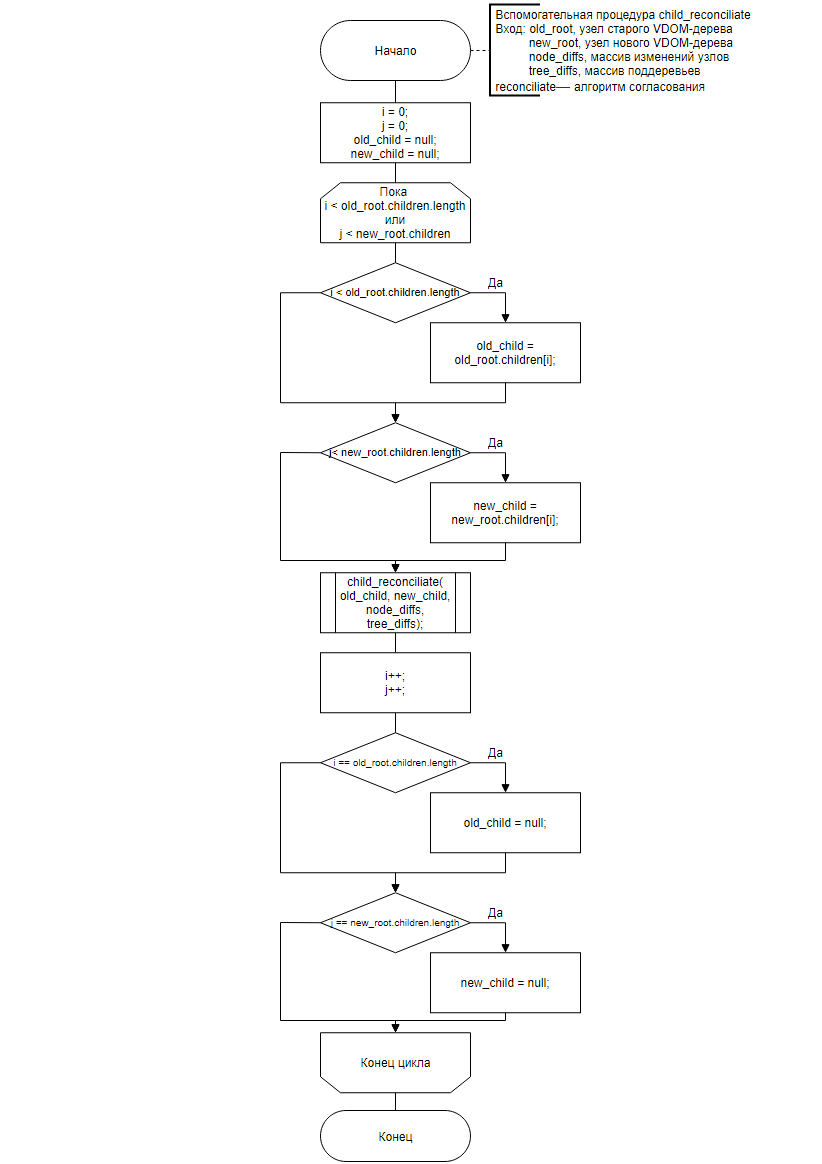
\includegraphics[width=170mm]{img/child-reconciliation-algorithm.png}
	\caption{Схема алгоритма согласования, часть 2}
	\label{fig:child-reconciliation-algorithm}
\end{figure}

\begin{figure}[h]
	\centering
	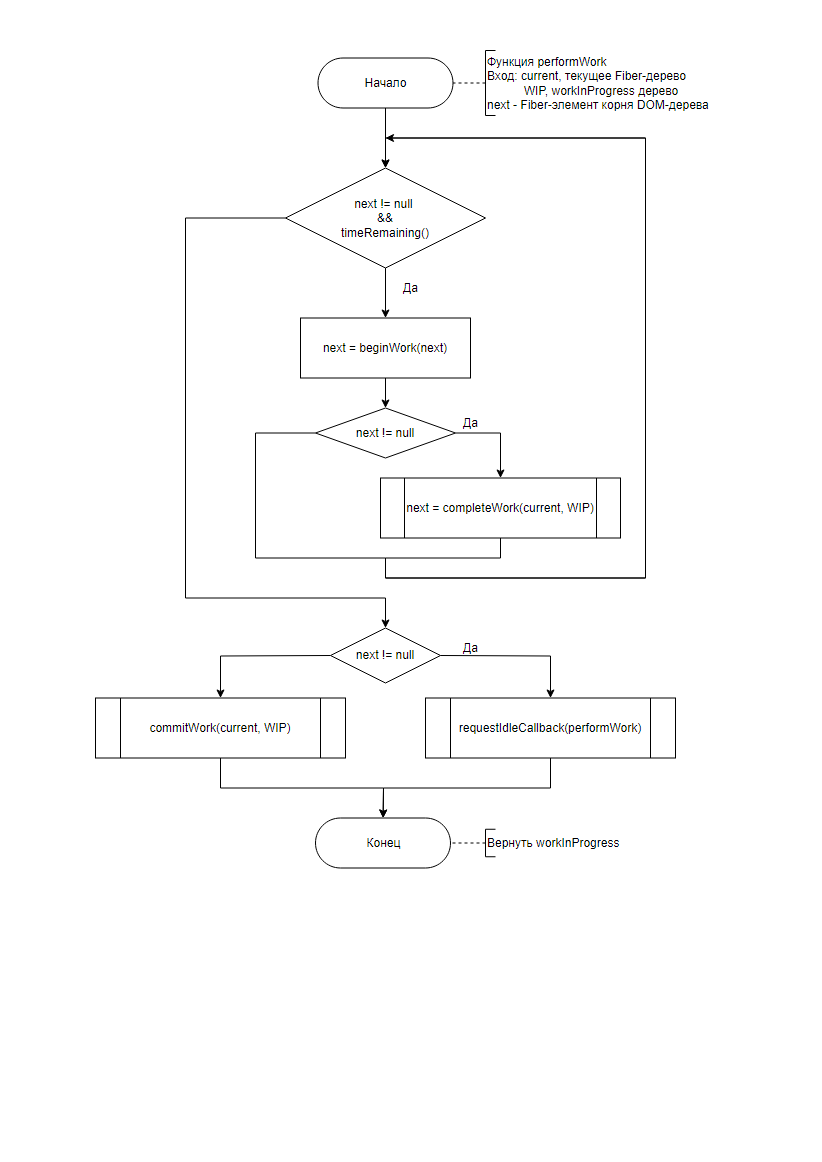
\includegraphics[width=170mm]{img/fiber-main.png}
	\caption{Схема алгоритма Fiber}
	\label{fig:fiber-main}
\end{figure}

\begin{figure}[h]
	\centering
	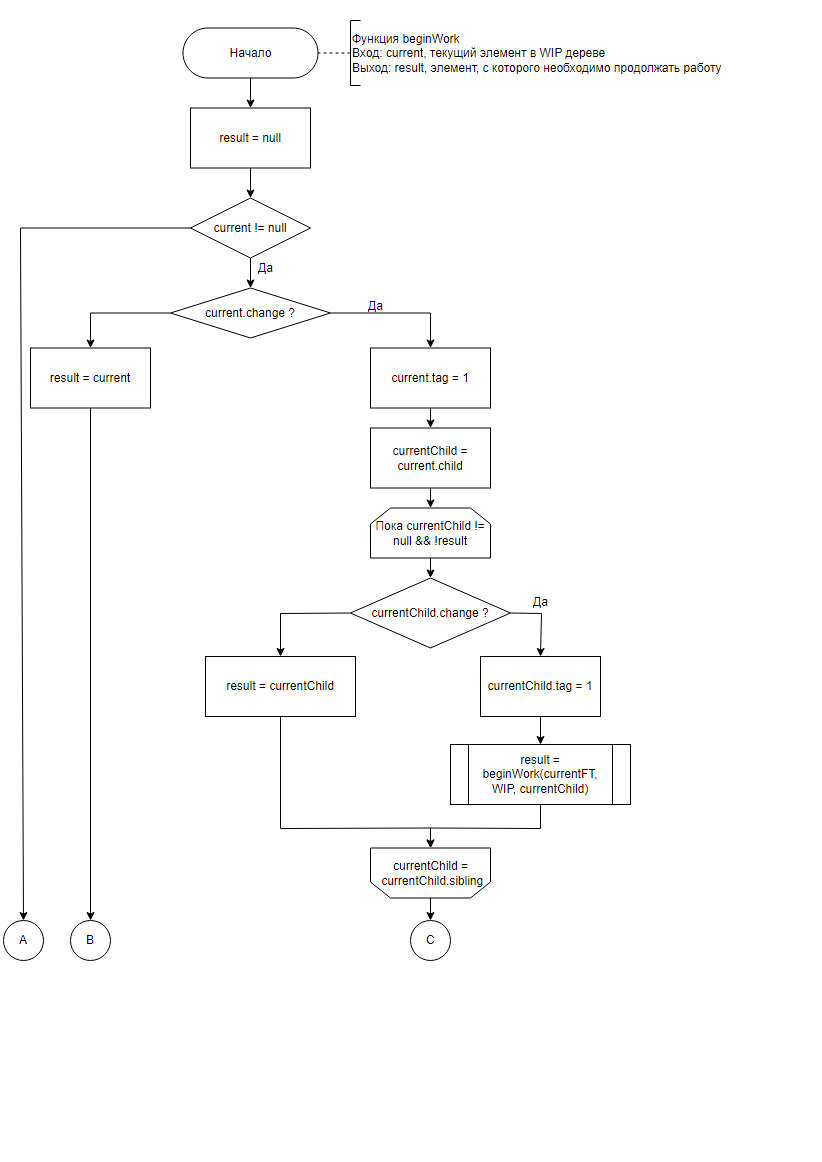
\includegraphics[width=170mm]{img/fiber-begin-work-1.png}
	\caption{Схема алгоритма функции beginWork, часть 1}
	\label{fig:fiber-begin-work-1}
\end{figure}

\begin{figure}[h]
	\centering
	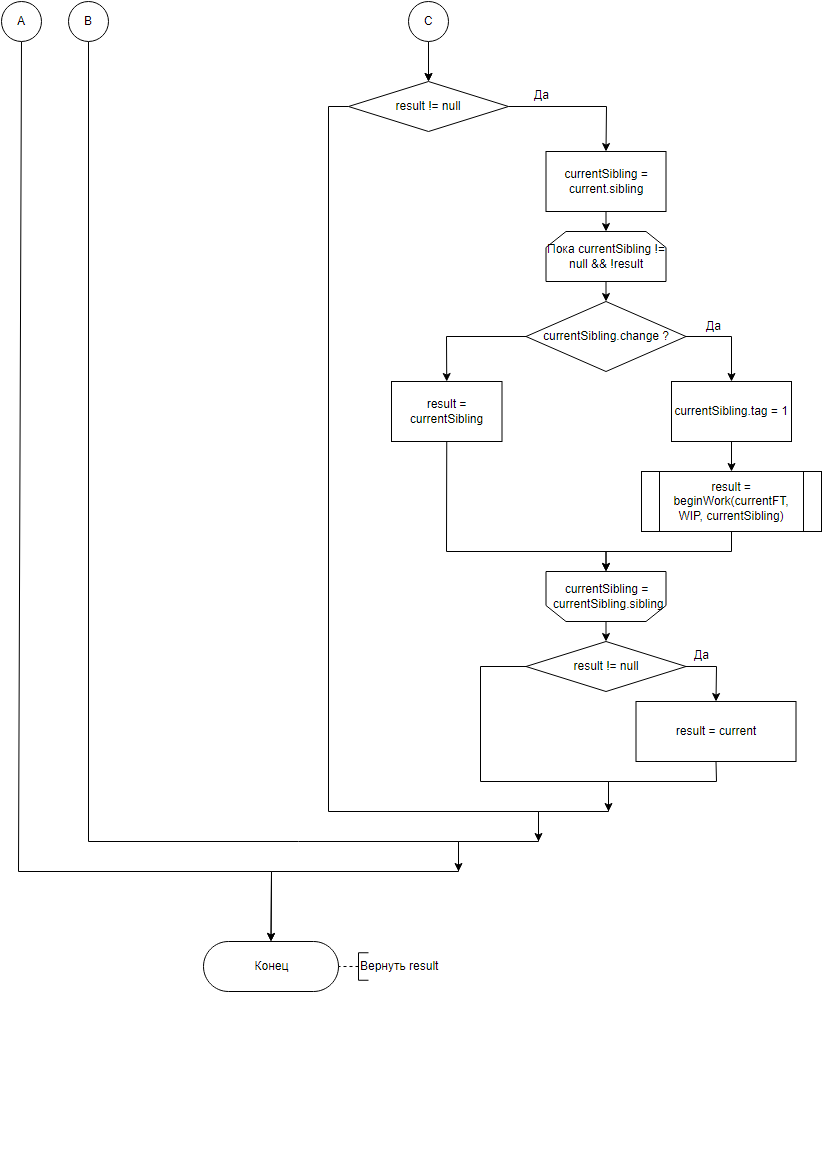
\includegraphics[width=170mm]{img/fiber-begin-work-2.png}
	\caption{Схема алгоритма функции beginWork, часть 2}
	\label{fig:fiber-begin-work-2}
\end{figure}

\begin{figure}[h]
	\centering
	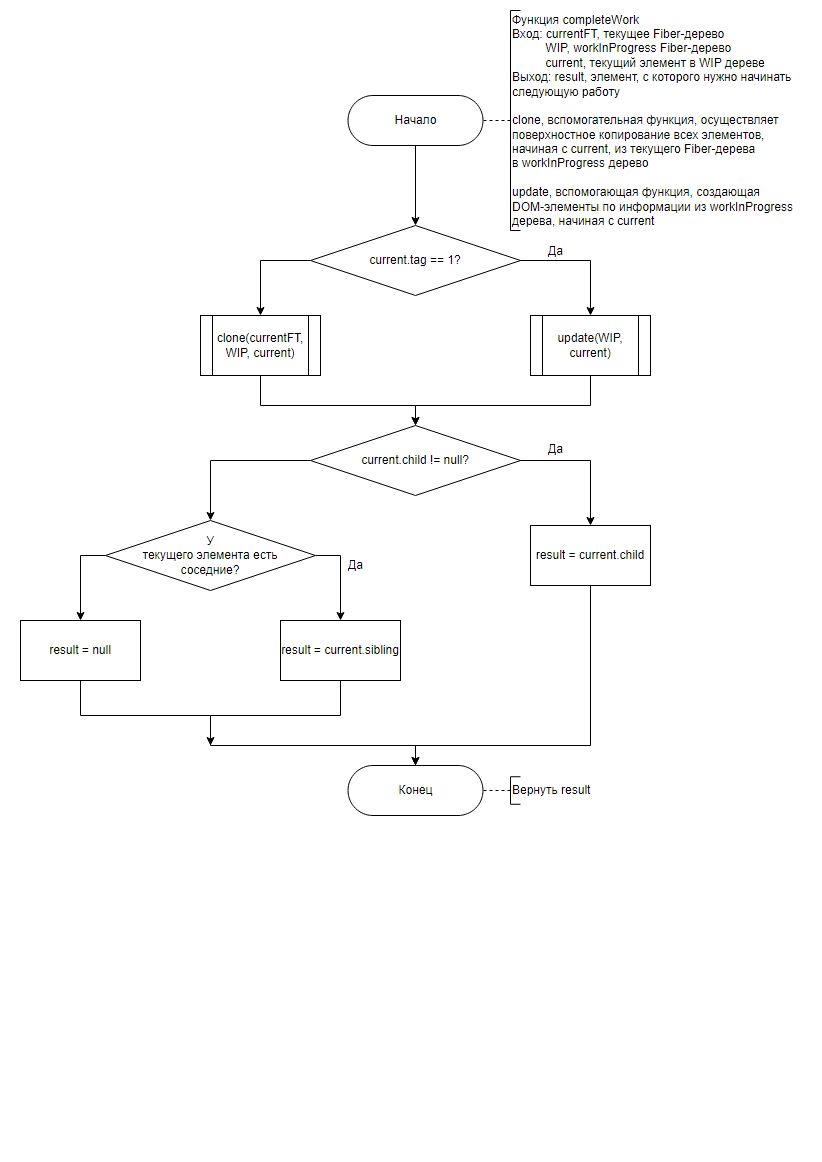
\includegraphics[width=170mm]{img/fiber-complete-work.png}
	\caption{Схема алгоритма функции completeWork}
	\label{fig:fiber-complete-work}
\end{figure}



\clearpage

\subsection{Модель вычислений для проведения оценки трудоёмкости}

Введем модель вычислений~\cite{model}, которая потребуется для определния трудоёмкости каждого отдельно взятого алгоритма.

\begin{enumerate}[label=\arabic*)]
	\item Операции из списка~(\ref{for:operations}) имеют трудоёмкость, равную 1.
	\begin{equation}
		\label{for:operations}
		+, -, /, *, \%, =, +=, -=, *=, ==, !=, <, >, <=, >=, [], ++, {-}-, . 
	\end{equation}
	\item Трудоёмкость оператора выбора \codeword{if условие then A else B} рассчитывается по формуле~(\ref{for:if}).
	\begin{equation}
		\label{for:if}
		f_{if} = f_{\text{условия}} +
		\begin{cases}
			f_A, & \text{если условие выполняется,}\\
			f_B, & \text{иначе.}
		\end{cases}
	\end{equation}
	\item Трудоёмкость цикла рассчитывается по формуле~(\ref{for:cycle}).
	\begin{equation}
		\label{for:cycle}
		f_{for} = f_{\text{инициализации}} + f_{\text{сравнения}} + N(f_{\text{тела}} + f_{\text{инкремент}} + f_{\text{сравнения}})
	\end{equation}
	\item Трудоёмкость вызова функции равна 0.
\end{enumerate}


\subsection{Трудоёмкость алгоритмов}

Определим трудоёмкость выбранных алгоритмов по их схемам согласно выбранной модели вычислений для оценки.

\subsubsection{Алгоритм обновления документа с использованием DOM}

Введём следующие обозначения:
\begin{enumerate}[label=\arabic*)]
	\item $n$ --- количество узлов в DOM-дереве;
	\item $old$ --- случайная величина, значение которой может быть 1 или 0 в зависимости от того, нужно ли менять значение узла на новое;
	\item $E(old)$ --- математическое ожидание случайной величины $old$;
	\item $x$ --- трудоёмкость операции \codeword{update}, $x >> 1$.
\end{enumerate}

Поскольку величина $old$ может принимать значение 1 только в случае одного узла и 0 во всех остальных случаях, можно найти значение её математического ожидания по формуле~(\ref{for:e-old}).
\begin{equation}
	\label{for:e-old}
	E(old) = 1 \cdot \frac{1}{n} + 0 \cdot \frac{n - 1}{n} = \frac{1}{n}
\end{equation}

Трудоёмкость алгоритма обновления документа с использованием DOM будет вычисляться по формуле~(\ref{for:f-dom-1}).
\begin{equation}
	\label{for:f-dom-1}
	f_{dom} = n \cdot (2 + 1 + E(old) + x + 2 + 3)
\end{equation}

C учётом формулы~(\ref{for:e-old}) получим итоговую формулу~(\ref{for:f-dom-2}) для расчёта трудоёмкости алгоритма обновления документа с использованием DOM.
\begin{equation}
	\label{for:f-dom-2}
	f_{dom} = xn + 8n + 1
\end{equation}

Поскольку $x >> 1$, $f_{dom} \approx \Theta(xn)$.

\subsubsection{Алгоритм обновления документа с использованием VDOM}
Введём следующие обозначения:
\begin{enumerate}[label=\arabic*)]
	\item $n$ --- количество узлов в изменяемом VDOM-дереве;
	\item $k$ --- случайная величина, которая может принимать значения от 0 до $n$ включительно в зависимости от того, в каком количестве узлов необходимо изменить содержимое;
	\item $E(k)$ --- математическое ожидание случайной величины $k$;
	\item $t$ --- случайная величина, которая может принимать значения от 0 до $n - k$ включительно в зависимости от того, какое количество поддеревьев требует полной перерисовки;
	\item $E(t)$ --- математическое ожидание случайной величины $t$;
	\item $x$ --- трудоёмкость операции \codeword{update}, $x >> 1$;
	\item $f_{reconciliate}$ --- трудоёмкость алгоритма согласования.
\end{enumerate}

Поскольку случайная величина $k$ принимает свои значения равновероятно, можно найти её математическое ожидание по формуле~(\ref{for:e-k}).
\begin{align}
	\begin{split}
		\label{for:e-k}
		E(k) &= \frac{n}{n + 1} + \frac{n - 1}{n + 1}  + \dotsc + \frac{1}{n + 1} + \frac{0}{n + 1} \\
		&= \frac{1}{n + 1} \cdot \frac{(n + 0)\cdot(n + 1)}{2} = \frac{n}{2}
	\end{split}
\end{align}

Аналогичным образом найдём математическое ожидание случайной величины $t$, формула~(\ref{for:e-t}).

\begin{align}
	\begin{split}
		\label{for:e-t}
		E(t) &= \frac{n - E(k)}{n - E(k) + 1} + \frac{n - E(k) - 1}{n - E(k) + 1} + \dotsc +  \frac{1}{n - E(k) + 1} \\
		&+\frac{0}{n - E(k) + 1} = \frac{1}{n - E(k) + 1} \cdot \frac{(n - E(k) + 0)\cdot(n - E(k) + 1)}{2}\\
		&= \frac{n - E(k)}{2} = \frac{n}{4}
	\end{split}
\end{align}

Трудоёмкость алгоритма обновления документа с использованием VDOM будет вычисляться по формуле~(\ref{for:f-dom-1}).
\begin{align}
	\begin{split}
	\label{for:f-vdom-1}
	f_{vdom} &= 2 + f_{reconciliate} + 2 + E(k)\cdot(3 + x) + 2 + E(t)\cdot(3 + f_{dom}) \\
	&= E(k) \cdot (x + 3) + E(t) \cdot (f_{dom} + 3) + 6
	\end{split}
\end{align}

С использованием формул~(\ref{for:e-k}) и~(\ref{for:e-t}) получим итоговую формулу~(\ref{for:f-vdom-2}) расчёта трудоёмкости алгоритма обновления документа с использованием VDOM.
\begin{equation}
	\label{for:f-vdom-2}
	f_{vdom} = \frac{n \cdot (3 + x)}{2} + \frac{n\cdot(3 + f_{dom})}{2} + f_{reconciliate} + 6
\end{equation}


\subsubsection{Алгоритм согласования}

Для алгоритма согласования рассмотрим худший и лучший случай.

Худшим случаем будем считать случай, при котором необходимо изменить все параметры всех узлов дерева, и добавить новые узлы в каждый из листовых узлов.
Введём следующие обозначения:
\begin{enumerate}[label=\arabic*)]
	\item $n$ --- количество узлов в изменяемом VDOM-дереве;
	\item $m$ --- количество параметров в одном узле;
	\item $k$ --- количество листов изменяемого VDOM-дерева;
	\item $\lambda$ --- количество новых узлов, добавлемых в каждый лист изменяемого VDOM-дерева.
\end{enumerate}

Тогда трудоёмкость алгоритма согласования для худшего случая может быть вычислена по формуле~(\ref{for:f-reconciliation-worst}).

\begin{align}
	\begin{split}
		\label{for:f-reconciliation-worst}
		f_{reconciliate_{worst}} &= (n + \lambda) \cdot (5 + 1 + 2 + m \cdot (3 + 2 + m \cdot (3 + 1 + 3)) \\
		&+ 2 + 7 + 4 + 4 + 7) + (n + \lambda) \cdot (2 + 2 + 2) + n \cdot 3 \\
		&+ (n + \lambda) \cdot 3 + \lambda + 1 =\\
		&= (n + \lambda) \cdot (41 + m \cdot (5 + 7m)) + 3n + \lambda + 1 \\
		&= (7m^2 + 5m)\cdot(n + \lambda) + 44n + 42\lambda + 1
	\end{split}
\end{align}

Лучшим случаем для алгоритма согласования будем считать случай, при котором разница в типе узла находится в первом же узле,~т.~е. возникает необходимость перерисовать всё дерево целиком, что является худшим случаем для алгоритма обновления документа с использованием VDOM и алгоритма согласования.

Трудоёмкость алгоритма согласования для лучшего случая считается по формуле~(\ref{for:f-reconciliation-best}).

\begin{align}
	\begin{split}
		\label{for:f-reconciliation-best}
		f_{reconciliate_{best}} &= 1 + 2 + 2 + 4 = 9
	\end{split}
\end{align}

\subsubsection{Алгоритм Fiber}

Для алгоритма Fiber рассмотрим худший и лучший случай, аналогично худшему и лучшему  случаю при анализе трудоёмкости алгоритма согласования.

Введём следующие обозначения:
\begin{enumerate}[label=\arabic*)]
	\item $n$ --- количество узлов в изменяемом (workInProgress) дереве;
	\item $m$ --- количество параметров в одном узле;
	\item $k$ --- количество листов workInProgress-дерева;
	\item $\lambda$ --- количество новых узлов, добавлемых в каждый лист изменяемого VDOM-дерева;
	\item $f_{r}$ --- суммарная трудоёмкость вызовов функции requestIdleCallback и \linebreak timeRemaining;
	\item $x$ --- трудоёмкость функции update (для обновления DOM-элементов);
	\item $f_{begin}$ --- суммарная трудоёмкость вызовов функции beginWork;
	\item $f_{complete}$ --- суммарная трудоёмкость вызовов функции completeWork;
	\item $f_{commit}$ --- трудоёмкость алгоритма, выполняемого во время фазы закрепления;
\end{enumerate}

Трудоёмкость алгоритма Fiber для худшего случая может быть вычислена по формуле \ref{for:f-fiber}.
\begin{align}
	\begin{split}
		\label{for:f-fiber}
		f_{fiber} &= 1 + f_ {r} + f_{begin} + f_{complete} + f_{commit}
	\end{split}
\end{align}

В худшем случае, суммарная трудоёмкость функций beginWork и \linebreak completeWork может быть вычислена по формулам \ref{for:f-begin-work-worst} и \ref{for:f-complete-work-worst}.
\begin{align}
	\begin{split}
		\label{for:f-begin-work-worst}
		f_{beginWork_{worst}} &= n \cdot(1 + 1 + 1 + 2 + 2 + 1 \cdot (1 + 1 + 2) + 2 + 1  + 1) +\\
&+ \lambda \cdot (1 + 1 + 1 + 2 + 2 + 1 + 1 + 1 + 2 + 1 + 1 + 1) \\
&= 15n + 15\lambda 
	\end{split}
\end{align}
\begin{align}
	\begin{split}
		\label{for:f-complete-work-worst}
		f_{completeWork_{worst}} &= n \cdot (m + 1 + 2 + 1) + k \cdot (x + 2 + 1 + 1 + 2 + 1) \\
&= mn + 4n + kx + 7k
	\end{split}
\end{align}

В лучшем случае, суммарная трудоёмкость функций beginWork и \linebreak completeWork может быть вычислена по формулам \ref{for:f-begin-work-best} и \ref{for:f-complete-work-best}.
\begin{align}
	\begin{split}
		\label{for:f-begin-work-best}
		f_{beginWork_{best}} &= n \cdot (1 + 2 + 1 + 1) = 5n
	\end{split}
\end{align}
\begin{align}
	\begin{split}
		\label{for:f-complete-work-best}
		f_{completeWork_{best}} &= n \cdot(2 + x)
	\end{split}
\end{align}

Трудоёмкость фазы закрепления $f_{commit}$ будет одинаковой и в лучшем, и в худшем случае, поскольку она представляет из себя перенос значений ссылок на DOM-элементы, отрисованные и хранящиеся в workInProgress дереве, в реальное DOM-дерево. Считая, что $n$ --- количество элементов workInProgress-дерева, будем считать, что $f_{commit} = n$ .

Трудоёмкость алгоритма Fiber для худшего случая считается по формуле \ref{for:f-fiber-worst}.
\begin{align}
	\begin{split}
		\label{for:f-fiber-worst}
		f_{fiber_{worst}} &= 1 + f_{r} + 15n + 15\lambda + mn + 4n + kx + 7k + n \\
		&= kx + mn + 20n + 7k + 15\lambda + 1
	\end{split}
\end{align}

C учётом того, что вызовы функций requestIdleCallback и timeRemaining обязаны выполняться в течении 1 мс  согласно стандарту W3C~\cite{requestidlecallback-recommended}, будем считать, что $1 < f_{r} << x$. Тогда трудоёмкость алгоритма Fiber для худшего случая может быть оценена по формуле \ref{for:f-fiber-worst-final}.
\begin{align}
	\begin{split}
		\label{for:f-fiber-worst-final}
		f_{fiber_{worst}} \approx \Theta(kx + mn)
	\end{split}
\end{align}

Трудоёмкость алгоритма Fiber для лучшего случая считается по формуле \ref{for:f-fiber-best} и может быть оценена по формуле 
\begin{align}
	\begin{split}
		\label{for:f-fiber-best}
		f_{fiber_{best}} &= 1 + f_{r} + f_{beginWork_{worst}} + f_{completeWork_{worst}} + f_{commit} =\\
		&= 1  + f_{r} + 5n + n\cdot(2 + x) + n = n  \cdot (x  + 8) + 1
	\end{split}
\end{align}
\begin{align}
	\begin{split}
		\label{for:f-fiber-best-final}
		f_{fiber_{worst}} \approx \Theta(xn)
	\end{split}
\end{align}

\subsection{Сравнение трудоёмкостей алгоритмов}

Сравним трудоёмкости алгоритмов обновления документа с использованием DOM и VDOM.

Трудоёмкость алгоритма обновления документа с использованием DOM была вычислена по формуле~(\ref{for:f-dom-2}) и не зависит только от двух параметров, являясь пропорциональной $\Theta(xn)$, где $x$ --- трудоёмкость операции update отрисовки узла, а $n$ --- количество узлов в новом DOM-дереве.

Трудоёмкость алгоритма обновления документа с использованием VDOM и алгоритма согласования зависит от того, насколько предположения, заложенные в основу эвристики алгоритма согласования, выполняются.

Так, если процесс изменения производится с учётом данных предположений, будет некорректно считать результат работы алгоритма согласования равновероятным, и, следовательно, считать трудоёмкость использующего его алгоритма обновления посредством VDOM через формулу~(\ref{for:f-vdom-2}). 
Однако трудоёмкость, вычисленная посредством формулы~(\ref{for:f-vdom-1}) остаётся верной, поэтому дальнейшие выводы будут сделаны, основываясь на данной формуле.

Чем лучше соблюдаются предположения, положенные в основу алгоритма согласования, чем меньше будет величина $t$,~т.~е. количество поддеревьев, требующих полной перерисовки. 
То есть трудоёмкость алгоритма будет пропорциональна $\Theta(xk)$, где $k$ --- количество узлов, требующих перерисовки, $k << n$ в общем случае.

Иными словами, алгоритм обновления документа с использованием\break VDOM и алгоритма согласования будет иметь меньшую трудоёмкость, чем алгоритм обновления документа с использованием DOM, за счёт понимания того, какие узлы нужно перерисовывать, а какие нет.

Стоит отметить, что при несоблюдении предположений, на которых основывается алгоритм согласование, трудоёмкость алгоритма с использованием VDOM будет превышать трудоёмкость алгоритма, использующего DOM. 
Такая ситуация произойдёт, например, при постоянном изменении типа корневого элемента.

Эвристика, применимая для алгоритма согласования, работает и в случае алгоритма Fiber. Трудоёмкость алгоритма Fiber в случае изменения типа первого элемента DOM-дерева (корня) может быть вычислена через по формуле \ref{for:f-fiber-best-final} и совпадает со значениям, полученными при рассмотрении аналогичных ситуаций для алгоритма обновления с использования DOM в формуле \ref{for:f-dom-2} и алгорима обновления, использующего согласование. В других случаях, в том числе при добавлении новых  элементов в каждый листовой элемент, трудоёмкость алгоритма Fiber будет пропорциональна $\Theta(kx + mn)$, что превышает значение, полученное выше для алгоритма обновления с использованием согласования на значение линейного члена $mn$. Тем не менее, алгоритм Fiber обеспечивает обновление лишь тех узлов, которые необходимо перерисовывать, как и алгоритм с использованием согласования.

\subsection{Сравнение алгоритмов по памяти}

Стандарт W3C для объектной модели документа гласит, что управление памятью зависит полностью от реализации~\cite{dom}, поэтому в данной работе уделяется внимание лишь дополнительной памяти, требуемой алгоритмами.

В случае алгоритма обновления документа с использованием VDOM и алгоритм согласования, дополнительной памятью будем считать оперативную память, используемую под хранение виртуальной объектной модели документа. Как и DOM, VDOM хранится в памяти в виде дерева элементов, содержащих всю необходимую для рендера соответствующих виртуальным элемента реальных элементов DOM.  В данной работе нет возможности исследовать точное потребление памяти алгоритмами, однако есть возможность сравнить потребление памяти относительно разных алгоритмов.

Использование VDOM может приводить к увеличению объёма дополнительную памяти в 5 раз по сравнению объёмом памяти, используемым в стандартном DOM алгоритме~\cite{memory-consumption}. Тем не менее, данные затраты считаются приемлимыми при использовании таких готовых решений, как React или Vue~\cite{vdom-overhead}.

В случае алгоритма Fiber, также относящегося к алгоритмам, использующим VDOM, память используется в меньших объёмах, чем при использовании алгоритма согласования~\cite{react-dive}. Это связано с тем, что объекты Fiber являются основными составляющими дерева, характеризующего объектнную модель документа. В этом дереве содержится информация, необходимая для рендера элементов в реальный DOM, в том числе ссылки на элементы реального DOM, соответствующие объектам Fiber. Это позволяет экономить память в случаях, когда необходимую информацию можно найти в объектах DOM~\cite{fiber-saves-memory}.

\subsection{Сравнение алгоритмов по пользовательскому опыту}

Основной недостаток алгоритма обновления документа с использованием DOM заключается в обновлении всех элементов DOM вне зависимости от того, является обновление необходимым или нет. Это приводит к тому, существует граничное значение количества элементов DOM, при превышении которого пользователь сможет заметить ''скачки'' из-за уменьшения количества кадров в секунду. Так, в браузере Google Chrome это значение значение условно отмечается как 1400~\cite{dom-max}, причём отмечается, что к таким же результатам может привести глубина DOM-дерева, превышающая значение 32.

Использование VDOM и алгоритма согласования решает эту проблему, обновляя лишь необходимые элементы. Тем не менее, при достаточно большом количестве обновляемых элементов данные вычисления будут занимать ощутимое для пользователя время, поскольку будут занимать время, превышающее 16.67 миллисекунд~\cite{react-dive}. Это происходит из-за того, что алгоритм обновления документа с использованием VDOM и алгоритм согласования выполняется от начала  до конца, блокируя тем самым выполнение других вычислений.

Данную проблему решает алгоритм Fiber. Фаза рендера, во время которой выполняется преимущественный объём вычислений, делится на множество частей при помощи функции requestIdleCallback. Благодаря этому даже при значительном объёме обновляемых элементов сохраняется плавность движения и количество кадров в секунду, большее 60~\cite{react-dive}.
\subsection*{Вывод}

Были разработаны схемы алгоритмов обновления гипертекстового документа с использованием DOM, VDOM и алгоритма согласования, а также алгоритма Fiber. Были найдены их трудоёмкости и произведено их сравнение по критериям, оописанным в аналитическом разделе.

Трудоёмкость алгоритма обновления документа с использованием DOM пропорциональна $\Theta(xn)$, где $x$ --- трудоёмкость операции update отрисовки узла, а $n$ --- количество узлов в новом DOM-дереве.
В это время трудоёмкость обновления документа с использованием VDOM и алгоритма согласования в случае соблюдения предположений, лежащих в основе алгоритма согласования, пропорциональна $\Theta(xk)$, где $k$ --- количество узлов, требующих перерисовки, $k << n$ в общем случае.
Трудоёмкость алгоритма Fiber при соблюдении аналогичных эвристических предположений пропроциональна $\Theta(xk + mn)$, где $m$ --- количество параметров, изменяемых при обновлении, $n$ --- количество узлов в DOM-дереве.

Из перечисленных алгоритмов именно алгоритм Fiber позволяет обеспечивать плавность обновления изображения на экране и при большом размере DOM-дерева, и при большом количестве операций обновления, в то время как алгоритм обновления с использованием алгоритма согласования выполняется от начала до конца и при большом количестве операций обновления может приводить к уменьшению количества кадров в секунду.
\pagebreak